% Created 2017-08-21 Mon 13:03
\documentclass[11pt]{article}
\usepackage[utf8]{inputenc}
\usepackage{lmodern}
\usepackage[T1]{fontenc}
\usepackage{fixltx2e}
\usepackage{graphicx}
\usepackage{longtable}
\usepackage{float}
\usepackage{wrapfig}
\usepackage{rotating}
\usepackage[normalem]{ulem}
\usepackage{amsmath}
\usepackage{textcomp}
\usepackage{marvosym}
\usepackage{wasysym}
\usepackage{amssymb}
\usepackage{amsmath}
\usepackage[version=3]{mhchem}
\usepackage{url}
\usepackage{underscore}
\usepackage{threeparttable}
\usepackage{tabulary}
\usepackage{parnotes}
\usepackage{comment}
\usepackage{multirow}
\usepackage{booktabs}
\usepackage[innermargin=0.5in,outermargin=0.5in,vmargin=0.5in]{geometry}
\usepackage[dvipsnames,svgnames,table]{xcolor}
\usepackage[linktocpage,pdfstartview=FitH,colorlinks,linkcolor=blue,anchorcolor=blue,citecolor=blue,filecolor=blue,menucolor=blue,urlcolor=blue,citebordercolor={0 1 0}]{hyperref}
\usepackage{attachfile}
\usepackage[svgnames]{xcolor}
\usepackage{helvet}
\renewcommand{\familydefault}{\sfdefault}
\usepackage[backend=biber,citestyle=nature,bibstyle=nature,hyperref=true,backref=false,url=false,natbib=true]{biblatex}
\addbibresource{bibliography.bib}
\usepackage{sectsty}
\usepackage{siunitx}
\sisetup{detect-all}
\sectionfont{\normalfont\fontfamily{phv}\bfseries}
\subsectionfont{\normalfont\fontfamily{phv}\selectfont}
\subsubsectionfont{\normalfont\fontfamily{phv}\selectfont}
\subsubsectionfont{\normalfont\fontfamily{phv}\selectfont}
\paragraphfont{\normalfont\fontfamily{phv}\selectfont}
\subparagraphfont{\normalfont\fontfamily{phv}\selectfont}
\usepackage[tikz]{bclogo}
\usepackage{stackengine}
\usepackage{scalerel}
\usepackage[svgnames]{xcolor}
\newcommand\dangersign[1][4ex]{\renewcommand\stacktype{L}\scaleto{\stackon[1pt]{\color{red}$\triangle$}{\tiny !}}{#1}}
\usepackage{graphicx}
\usepackage{wrapfig}
\usepackage{tikz}
\def\checkmark{\tikz\fill[scale=0.3](0,.35) -- (.25,0) -- (1,.7) -- (.25,.15) -- cycle;}
\usepackage{fancyhdr}
\pagestyle{fancy}
\lhead{\ttfamily{v0.9 \date{\today}}}
\rhead{}
\renewcommand{\headrulewidth}{0pt}
\setcounter{secnumdepth}{4}
\author{David R. Hill\(^{\text{1*}}\), Sha Huang\(^{\text{1}}\), Yu-Hwai Tsai\(^{\text{1}}\), Jason R. Spence\(^{\text{1,2}}\), and Vincent B. Young\(^{\text{1,3}}\) \\\\\(^{\text{1}}\)Department of Internal Medicine, Division of Gastroenterology\\\(^{\text{2}}\)Department of Cell and Developmental Biology\\\(^{\text{3}}\)Department of Internal Medicine, Division of Infectious Disease\\ University of Michigan, Ann Arbor MI 48109\\\\\(^{\text{*}}\)Corresponding author (Email: hilldr@med.umich.edu; Tel: (440) 832 0000)}
\date{\today}
\title{\textbf{Real-time measurement of epithelial barrier permeability in human intestinal organoids}}
\begin{document}

\maketitle
\section*{SUMMARY}
This protocol describes the measurement of epithelial barrier permeability in real-time following pharmacologic treatment in human intestinal organoids using fluorescent microscopy and live cell microscopy.\\

\section*{ABSTRACT}
Advances in 3D culture of intestinal tissues obtained through biopsy or generated from pluripotent stem cells via directed differentiation have resulted in sophisticated \emph{in vitro} models of the intestinal mucosa. Leveraging these emerging model systems will require adaptation of tools and techniques developed for 2D culture systems and animals. Here, we describe a technique for measuring epithelial barrier permeability in human intestinal organoids in real-time. This is accomplished by microinjection of fluorescently-labeled dextran and imaging on an inverted microscope fitted with epifluorescent filters. Real-time measurement of the barrier permeability in intestinal organoids facilitates the generation of high-resolution temporal data in human intestinal epithelial tissue, although this technique is can also be applied to fixed timepoint imaging approaches. This protocol is readily adaptable for the measurement of epithelial barrier permeability following exposure to phamacologic agents, bacterial products or toxins, or live microorganisms.  With minor modifications, this protocol can also serve as a general primer on microinjection of intestinal organoids and users may choose to supplement this protocol with additional or alternative downstream applications following microinjection.\\

\section*{INTRODUCTION}
The intestinal epithelium forms a selective barrier that mediates the directional transport of nutrients, H\(_{\text{2}}\)O, ions, and waste products while minimizing nonspecific diffusion-mediated exchange of other particles between the lumen and the mesenchymal tissue or blood supply \supercite{standring2008gray,Buckley:2017}. The nonspecific permeability of the intestinal epithelial barrier has long been considered a key functional parameter in both health and disease \supercite{Clayburgh:2004,Turner:2009,Bischoff:2014,Odenwald:2017} that reflects the rate of diffusion of small molecules across the epithelium via the paracellular space. Measurement of epithelial barrier permeability can be conducted in animal models \supercite{Krugliak:1994} and in human patients \supercite{Johnston:2001} through the ingestion of lactulose, which has no specific transporter in the gastrointestinal tract, and the subsequent collection and measurement of lactulose concentrations in peripheral blood. Alternate ingested markers of barrier function such as fluorescently labeled carbohydrates are also available \supercite{Salles_Teixeira:2014,Wang:2015}. This approach has been adapted for intestinal epithelial cell cultures grown on Transwell supports \supercite{Donato:2011}, a simplified approach that allows for greater experimental control but has also been criticized as a poor predictor of \emph{in vivo} permeability  due to the absence of differentiated epithelial subtypes and tissue structure \supercite{Balimane:2005}. Ussing chambers represent yet another approach and allow for the measurement of epithelial barrier function in whole intestinal mucosa \emph{ex vivo} \supercite{Vidyasagar:2016}. Application of this technique is frequently limited by tissue availability and condition \supercite{Vidyasagar:2016,Herrmann:2016}. Thus new methods which balance reproducibility and throughput with physiologic relevance are necessary.\\

Recent developments in \emph{in vitro} organogenesis have led to the adoption of 3D tissue culture model systems as a sophisticated platform for recapitulating the dynamics of complex tissues \supercite{Sato:2009,Clevers:2016,Drost:2016,Rookmaaker:2015,Spence:2011,Aurora:2016,Dedhia:2016,Dye:2015,Dye:2016}. In particular, human pluripotent stem cell (hPSC) derived human intestinal organoids (HIOs) \supercite{Spence:2011,McCracken:2011} have emerged as a reproducible and experimentally tractable model system for the study of host-microbial interactions and epithelial barrier dynamics \supercite{Leslie:2015,Leslie:2016,Zachos:2016, Hill:2017}. Similarly, human tissue-derived organoids (also know an enteroids) can be derived from a simple biopsy procedure and can be used as a tractable system to study human physiology and disease \supercite{Sato:2009,Miyoshi:2013,Sato:2011} Microinjection of human intestinal organoids allows for the delivery of experimental compounds \supercite{Leslie:2015} or live microbes \supercite{Engevik:2013, Leslie:2015,Forbester:2015,Engevik:2015} to the apical epithelial surface of the organoid lumen. Leslie and Huang \emph{et al.}\supercite{Leslie:2015} recently adapted this technique to measure barrier permeability in HIOs microinjected with fluorescein isothiocyanate (FITC) labeled dextran following exposure to bacterial toxins.\\

This protocol is intended as a guide for the measurement of epithelial barrier permeability in hPSC-derived HIOs and tissue-derived HIOs using fluorescent microscopy. With minor modifications, it can also serve as a general primer on microinjection of HIOs with experimental compounds. Users may supplement this protocol with additional or alternative downstream applications after microinjection.\\

\section*{PROTOCOL}
\section{{\bfseries\sffamily } Microinjector setup}
\label{sec:orgheadline10}
\subsection{{\bfseries\sffamily } Gather the materials listed in "Required Reagents".}
\label{sec:orgheadline1}
\subsection{{\bfseries\sffamily } Place the micromanipulator, dissecting scope, and light source in the biosafety cabinet. An example of a complete microinjector assembly is shown in \textbf{Figure 1}}
\label{sec:orgheadline2}
\begin{figure}
\centering
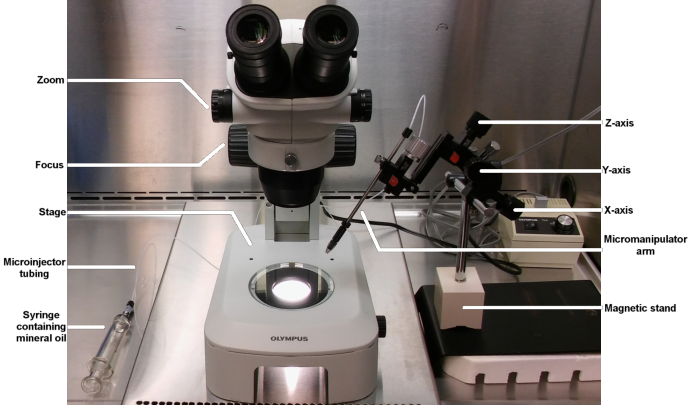
\includegraphics[width=0.9\linewidth]{./img/figure1.pdf}
\caption{Basic layout of a microinjector and micromanipulator for HIO microinjection.}
\end{figure}
\subsection{{\bfseries\sffamily } Position the dissecting scope so that the eye piece can be used through the access port.}
\label{sec:orgheadline3}
\begin{bclogo}[logo=\bcinfo, couleurBarre=Black, noborder=true, couleur=gray!10]{     Alternate setup}
A clean bench with positive air flow system may be used in place of a biosafety cabinet with microscope access points.\\
\end{bclogo}
\subsection{{\bfseries\sffamily } Assemble the micromanipulator on the right side of the microscope and adjust so that the controls can be easily reached and adjusted. The micromanipulator should be mounted on an iron plate or otherwise stabilized.}
\label{sec:orgheadline4}
\begin{bclogo}[logo=\bcinfo, couleurBarre=Black, noborder=true, couleur=gray!10]{     Lefties}
Left-handed users may want to place the micromanipulator to the left of the dissecting scope.\\
\end{bclogo}
\subsection{{\bfseries\sffamily } Mount the Micropipette Holder to the micromanipulator arm and connect the analog tubing.}
\label{sec:orgheadline5}
\subsection{{\bfseries\sffamily } Fill the 10 ml glass syringe with approximately 5-7 ml of sterile mineral oil.}
\label{sec:orgheadline6}
\subsection{{\bfseries\sffamily } Connect the 10ml glass syringe filled with mineral oil to the open end of the analog tubing. Place the glass syringe to the left of the dissecting scope, opposite from the micromanipulator.}
\label{sec:orgheadline7}
\subsection{{\bfseries\sffamily } Gently depress the syringe, pushing mineral oil through the tubing. Flush 10-20 drops of mineral oil from the tip of the micropipette holder. This step removes all air from the tubing and should be performed before each microinjection session.}
\label{sec:orgheadline8}
\subsection{{\bfseries\sffamily } Clean the microinjection setup with 70\% ethanol or other disinfectant prior to experimental use. Avoid prolonged exposure to disinfectants containing bleach, which may corrode the microinjection equipment.}
\label{sec:orgheadline9}
\section{{\bfseries\sffamily } Preparation for microinjection}
\label{sec:orgheadline42}

\subsection{{\bfseries\sffamily } 24 hours prior to microinjection:}
\label{sec:orgheadline13}
\subsubsection{{\bfseries\sffamily } Prepare FITC dextran solution by re-suspending FITC dextran at a concentration of 2 mg/ml in sterile PBS or saline. Prepare a total volume of > 250 \(\mu\)L}
\label{sec:orgheadline11}
\begin{bclogo}[logo=\bcinfo, couleurBarre=Black, noborder=true, couleur=gray!10]{     FITC dextran concentration}
Higher or lower concentrations of FITC-dextran may be used, ranging from approximately 0.1 - 10 mg/ml. Adjust the concentration of FITC-dextran to suit downstream the imaging application.\\
\end{bclogo}

\subsubsection{{\bfseries\sffamily } Setup organoid cultures on 4- or 8-well glass chamber slides or other culture vessel suitable for live microscopy, with up to 4-6 HIOs per well, embedded in 50 \(\mu\)l matrigel and cultured in ENR media. Take care to space the organoids evenly so as to avoid capturing multiple HIOs in a single microscopic field during real-time imaging analysis.}
\label{sec:orgheadline12}
\begin{bclogo}[logo=\bcinfo, couleurBarre=Black, noborder=true, couleur=gray!10]{     Use of tissue-derived HIOs}
This protocol was developed using stem-cell derived HIOs and the representative results (see below) demonstrate the use of this tissue culture model. However, the same protocol is easily adapted to tissue-derived intestinal epithelial organoids \supercite{Sato:2009,Miyoshi:2013}. A representative image demonstrating microinjection of tissue-derived intestinal epithelial organoids is shown in \textbf{Figure 3}. Tissue-derived HIOs are typically smaller than PSC-derived HIOs and lack the supporting mesenchymal basolateral cell structure\supercite{Sato:2009,Miyoshi:2013,Sato:2011}. Microinjection of tissue-derived HIOs may require a greater degree of technical ability and experience. The degree to which epithelial barrier permeability data obtained using tissue-derived HIOs may correlate with hPSC-derived HIOs is unknown.\\
\end{bclogo}

\subsection{{\bfseries\sffamily } At 30 minutes prior to microinjection, turn on the biosafety cabinet and raise the glass shield to the optimal working height}
\label{sec:orgheadline14}
\subsection{{\bfseries\sffamily } Before removing your HIOs from culture perform the following tasks:}
\label{sec:orgheadline41}
\subsubsection{{\bfseries\sffamily } Remove all unnecessary items from the biosafety cabinet. Clutter increases the risk of spills or other accidents when working in confined spaces.}
\label{sec:orgheadline15}
\subsubsection{{\bfseries\sffamily } Spray and thoroughly clean the work surface with 70\% ethanol or other disinfectant. Wipe clean using a paper towel.}
\label{sec:orgheadline16}
\subsubsection{{\bfseries\sffamily } Check the level of mineral oil in the glass syringe attached to the microinjector. If there is less than 3 mL of mineral oil remaining unscrew the syringe and refill inside the biosafety cabinet, being careful to avoid introducing bubbles. Do not fill more than 7 ml.}
\label{sec:orgheadline17}
\subsubsection{{\bfseries\sffamily } Turn on the lamp to illuminate the dissecting scope. Adjust the eyepiece for personal comfort.}
\label{sec:orgheadline18}
\subsubsection{{\bfseries\sffamily } Position the micromanipulator to the right of the dissecting scope. The micromanipulator is secured to an iron plate using a magnetic stand. Switch the magnetic stand to the OFF position to adjust the position of the micromanipulator and secure the stand to the iron plate by setting the magnetic stand to the ON position.}
\label{sec:orgheadline19}
\subsubsection{{\bfseries\sffamily } Microcapillary installation}
\label{sec:orgheadline40}
\paragraph{{\bfseries\sffamily } Retrieve a single glass filament from the 15 ml tube next to the micropippette puller.}
\label{sec:orgheadline20}
\paragraph{{\bfseries\sffamily } Thread the glass filament through the copper heating coil of the micropippette puller. See \textbf{Figure 2} for a guide to preparing the micropippette puller.}
\label{sec:orgheadline21}

\begin{figure}
\centering
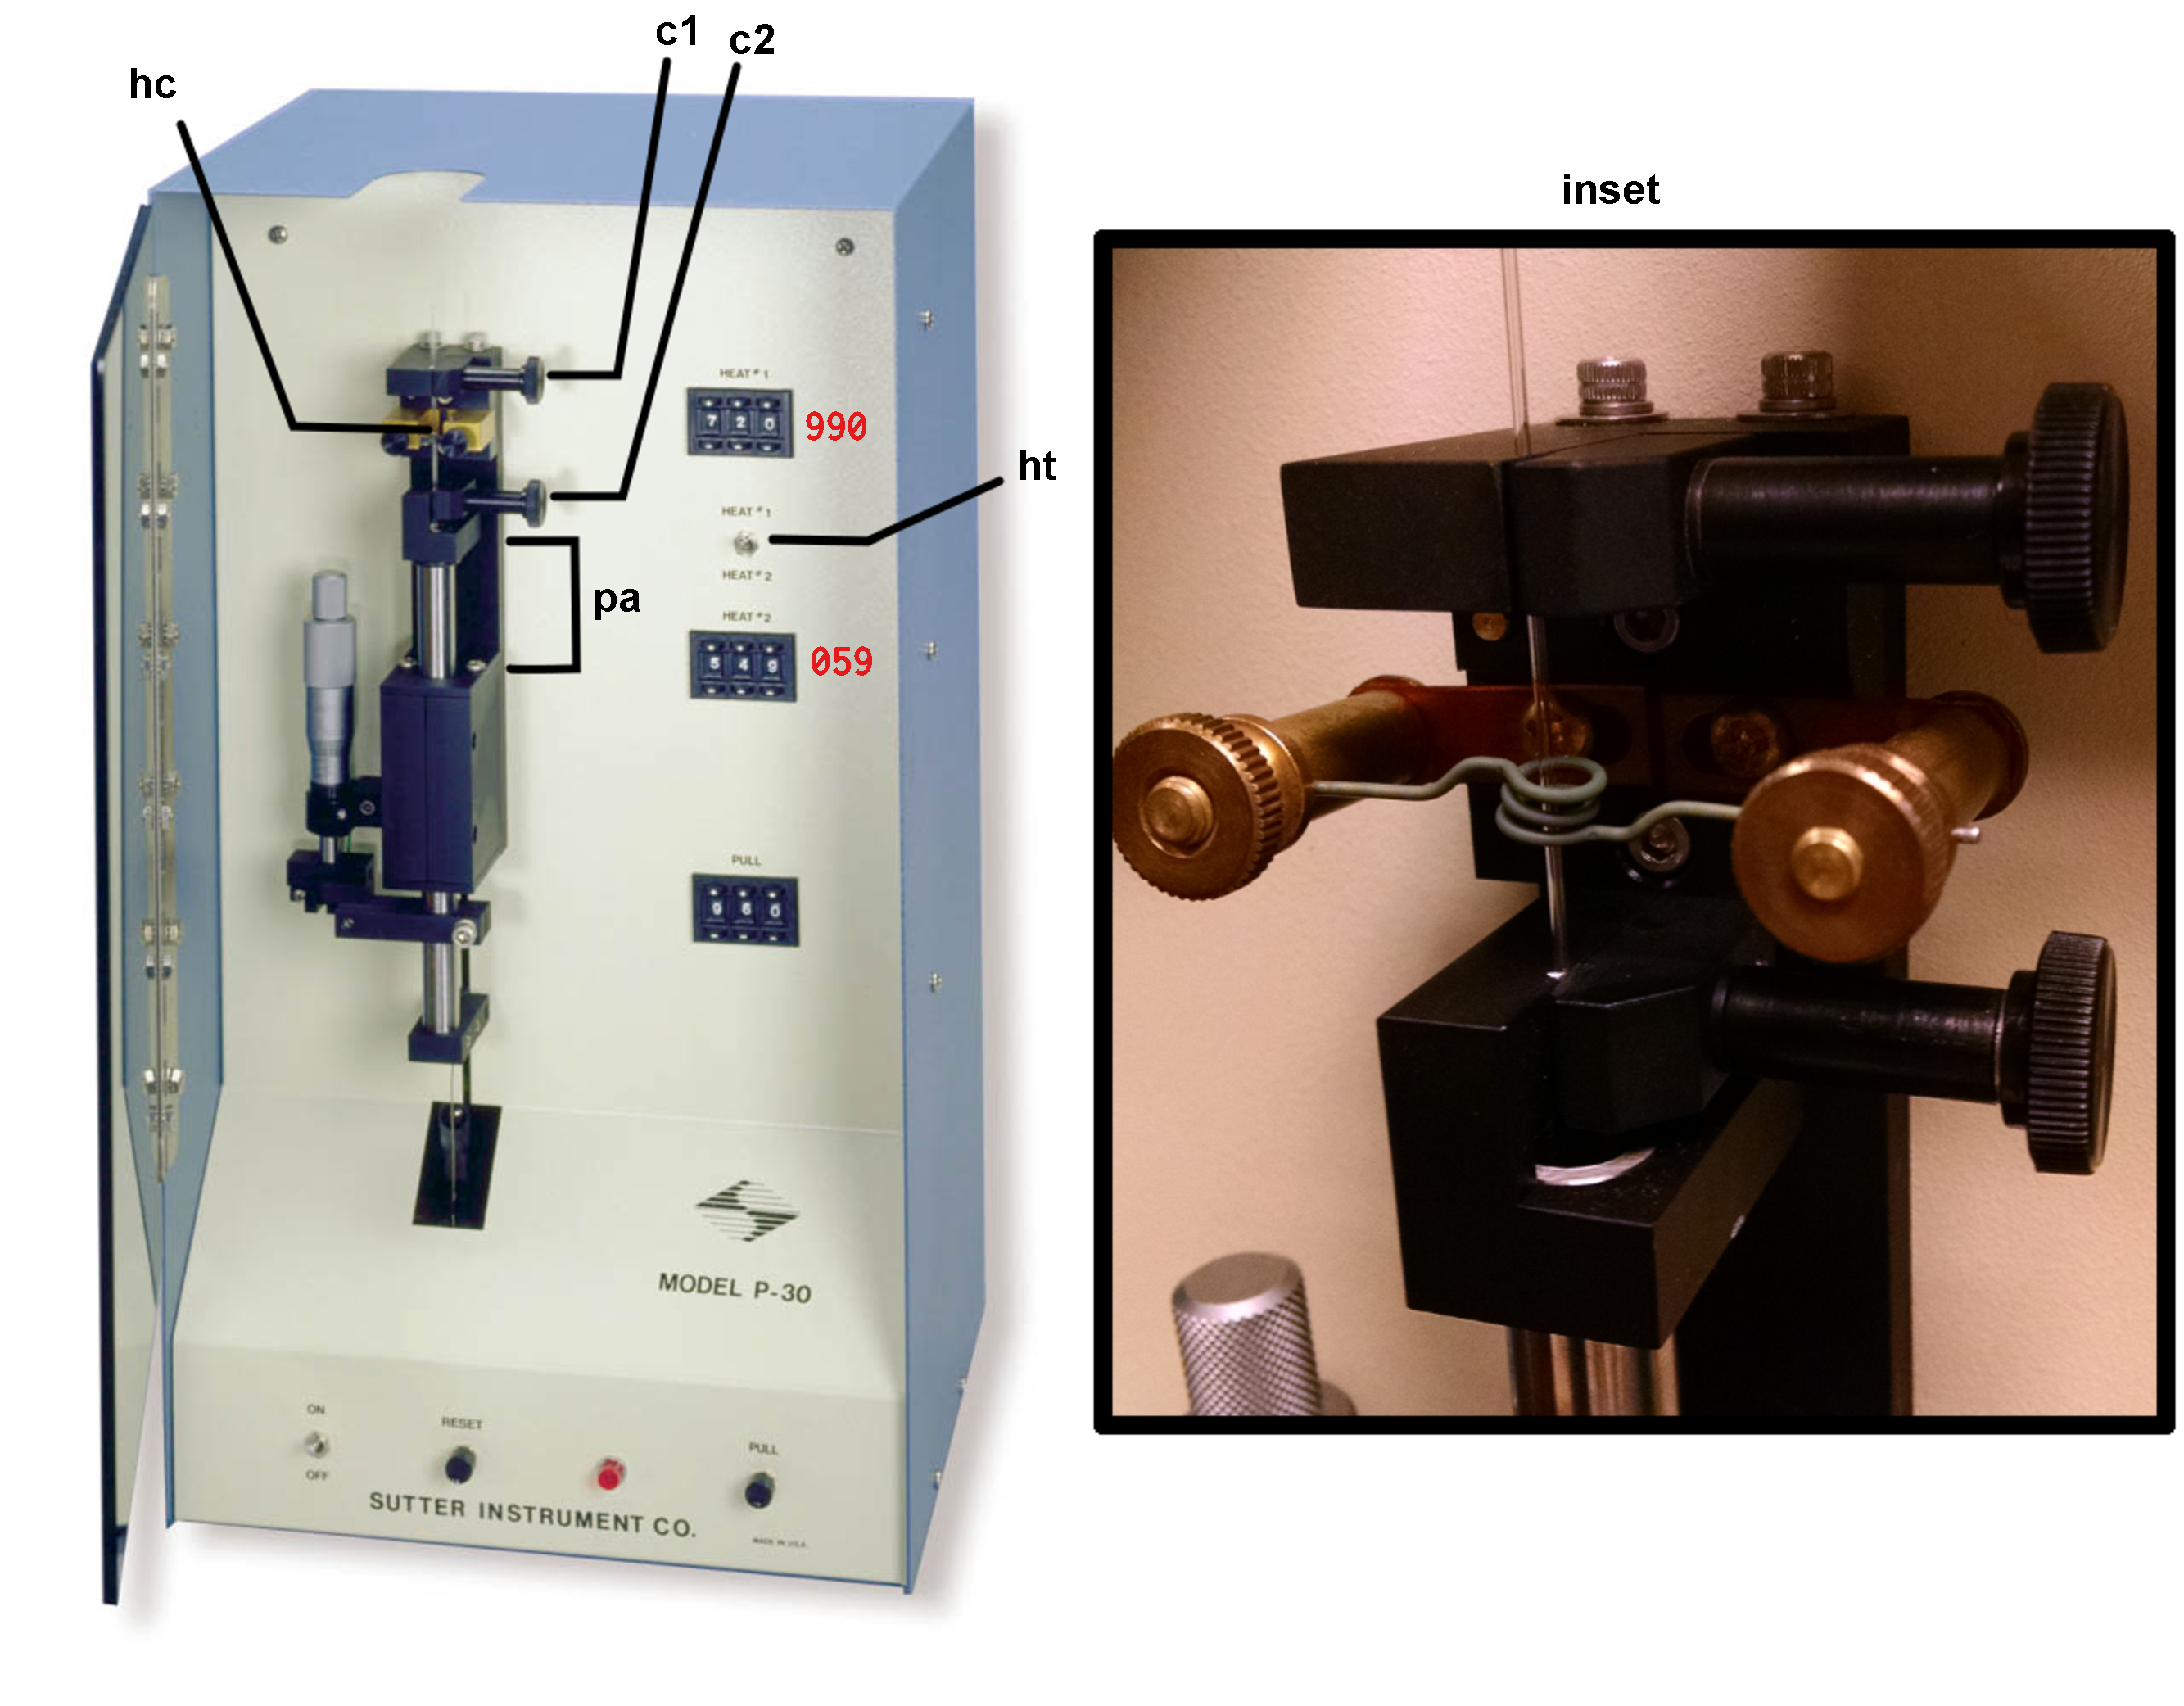
\includegraphics[width=0.6\linewidth]{./img/figure2.pdf}
\caption{Sutter Instrument Co. P-30 Micropipette puller. The copper heating coil \textbf{hc}, top clamp \textbf{c1}, bottom clamp (\textbf{c2}), puller arm (\textbf{pa}), heat selection toggle (\textbf{ht}) are identified by the arrows. The correct setting for HEAT 1 and PULL are indicated in red text. The \textbf{inset} shows a correctly mounted glass microcapillary ready for heating.}
\end{figure}

\paragraph{{\bfseries\sffamily } Secure the glass filament using the clamps.}
\label{sec:orgheadline22}
\paragraph{{\bfseries\sffamily } Position the filament so that the copper heating coil is approximately in the middle of the glass filament. This will ensure that the puller generates two usable microinjection needles from each glass filament.}
\label{sec:orgheadline23}
\paragraph{{\bfseries\sffamily } Tighten the top clamp first, making sure that the glass capillary is secured within the notched grove to prevent breakage.}
\label{sec:orgheadline24}
\paragraph{{\bfseries\sffamily } Extend the puller arm to its maximum vertical position before tightening the bottom clamp. \textbf{\emph{This step is essential}}. Failure to fully extend the puller arm will result in irregular separation of the two sections of the glass filament.}
\label{sec:orgheadline25}
\paragraph{{\bfseries\sffamily } Check the settings on the heating and pulling mechanism. Heat \#1 should be selected with the toggle. HEAT \#1 should read 990 and PULL should be set at 059.}
\label{sec:orgheadline26}
\paragraph{{\bfseries\sffamily } Turn on the instrument using the On/Off toggle.}
\label{sec:orgheadline27}
\paragraph{{\bfseries\sffamily } Close the protective plexiglass shield and press the PULL button on the bottom right face of the puller. The copper coil will begin to heat and will glow bright orange. As the temperature rises, the glass capillary will begin to stretch and eventually separate. Upon separation of the two ends of the glass filament, the instrument will power down.\\}
\label{sec:orgheadline28}
\begin{bclogo}[logo=\dangersign, couleurBarre=red, noborder=true, couleur=yellow!20]{     DANGER: Extreme heat}
The copper coil is extremely hot. Stand clear and wait approximately 30 s after separation of the glass filaments before handling.\\
\end{bclogo}
\paragraph{{\bfseries\sffamily } Being careful to avoid touching the copper coil, remove a one of the glass microinjection capillaries. The capillary should have a very fine point. Handle the capillary carefully with gloves and immediately proceed to the biosafety cabinet containing the microinjector setup. \\}
\label{sec:orgheadline29}
\begin{bclogo}[logo=\dangersign, couleurBarre=red, noborder=true, couleur=yellow!20]{     DANGER: Sharp point}
The glass microcapillary is extremely sharp. Handle with care.\\
\end{bclogo}
\paragraph{{\bfseries\sffamily } Insert the blunt end of the pulled microcapillary into the open end of the Micropipette Holder}
\label{sec:orgheadline30}
\paragraph{{\bfseries\sffamily } Secure the microcapillary to the Micropipette Holder by turning the screw clamp. Do not over-tighten the screw clamp.}
\label{sec:orgheadline31}
\paragraph{{\bfseries\sffamily } Ensure that the Micropipette Holder is positioned within the micromanipulator arm in such a way that it is stabilized by the grooved slot on the top face. \emph{Failure to correctly secure the microcapillary can result in instability or breakage of the microcapillary during microinjection}.}
\label{sec:orgheadline32}
\paragraph{{\bfseries\sffamily } Open the tip of the microcapillary needle. During preparation of the pulled microcapillary needle glass at the tip of the point will likely melt in such a way as to seal the pointed end of the microcapillary. To remove this blockage:}
\label{sec:orgheadline33}
\paragraph{{\bfseries\sffamily } Position the micromanipulator such that the microcapillary is pointed down at the glass stage of the dissecting scope without touching this surface.}
\label{sec:orgheadline34}
\paragraph{{\bfseries\sffamily } Find a sterile plastic surface (the underside of a culture plate lid works perfectly) and place it on the microscope stage directly underneath the microcapillary needle.}
\label{sec:orgheadline35}
\paragraph{{\bfseries\sffamily } Center the tip of the microcapillary under the viewing area and ensure that it is visible when looking through the eyepiece of the microscope.}
\label{sec:orgheadline36}
\paragraph{{\bfseries\sffamily } Using the micromanipulator controls, slowly advance the micromanipulator arm and microcapillary towards the sterile plastic culture lid until the tip barely contacts the plastic surface. This should be sufficient to induce a small break at the tip of the needle.}
\label{sec:orgheadline37}
\paragraph{{\bfseries\sffamily } Back the microcapillary away from the sterile surface to minimize the chance of accidental breakage before proceeding.}
\label{sec:orgheadline38}
\paragraph{{\bfseries\sffamily } Check microcapillary for flow by depressing the glass syringe, pushing mineral oil through the tubing. If the end of the microcapillary has been opened you will see a small droplet of mineral oil emerge from the tip of the microcapillary after a few seconds. If this does not occur, repeat the previous step and re-test. Aim for the smallest possible break that allows for fluid flow from the microcapillary in order to minimize the damage to the HIO during microinjection.}
\label{sec:orgheadline39}



\section{{\bfseries\sffamily } Sterile microinjection}
\label{sec:orgheadline57}
Once the microcapillary has been prepared, installed, and tested you may begin microinjecting HIOs. \textbf{Figure 2} illustrates a tissue-derived HIO that has been successfully injected with FITC-dextran.\\
\begin{figure}
\centering
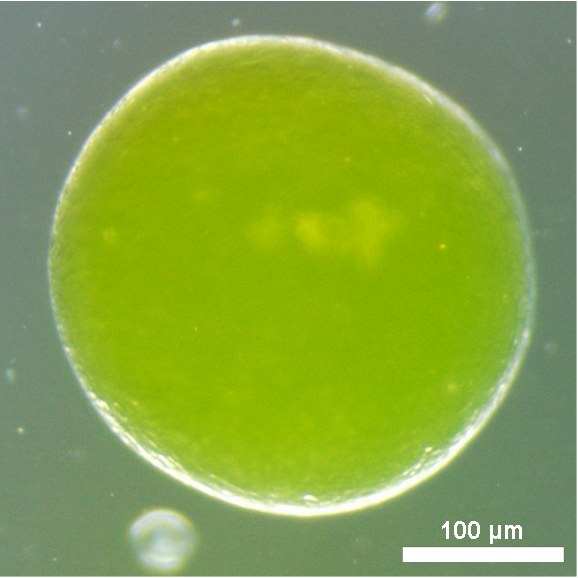
\includegraphics[width=0.35\linewidth]{./img/figure3.pdf}
\caption{Brightfield image of a tissue-derived human intestinal organoids after microinjection of FITC-dextran. Note that the fluorescence signal is apparent even without the use of a specific filter set. This coloration aids microinjection precision. 3X magnification}
\end{figure}

\subsection{{\bfseries\sffamily } Fill the microcapillary with your injection material. Submerge the microcapillary in the injection suspension, being careful to avoid breaking the tip of the microcapillary against the sides or bottom of the tube. Once the microcapillary is submerged in the solution, pull back on the mineral oil syringe to draw your suspension into the microcapillary}
\label{sec:orgheadline43}
\begin{bclogo}[logo=\bcinfo, couleurBarre=Black, noborder=true, couleur=gray!10]{     Preparing your suspension}
It is recommended that you use 1.5 mL or 0.5 mL eppendorf tubes for your injection solutions/cultures since these will be the most easily accessible to the installed microcapillary. If the suspension is highly viscous or if the opening of the microcapillary is exceptionally small, it may take several second to fill the microcapillary. Do not draw microinjection suspensions into the plastic microinjection tubing as this may contaminate the entire microinjection system.\\
\end{bclogo}

\subsection{{\bfseries\sffamily } Stop filling the microcapillary when your microinjection suspension fills 90\% of the length of the glass microcapillary. Depress the syringe slightly before withdrawing the microcapillary from the microinjection solution to ensure that the tip of the microcapillary does not contain pockets of air. If the examination of the microcapillary reveals pockets of air, empty and re-fill.}
\label{sec:orgheadline44}
\subsection{{\bfseries\sffamily } Remove your HIO culture plate(s) from the cell culture incubator and transfer to the biosafety cabinet with the microinjector.}
\label{sec:orgheadline45}
\subsection{{\bfseries\sffamily } Remove the lid from your HIO culture plate within the biosafety cabinet and center the first well on the microscope stage so that it is clearly visible through the eyepiece of the scope at the lowest magnification setting.}
\label{sec:orgheadline46}
\subsection{{\bfseries\sffamily } Position the micromanipulator arm such that the microcapillary is pointed down into the HIO culture well at an angle >45\textdegree{} relative to the microscope stage. This is most easily accomplished by manually turning the entire manipulator assembly on its horizontal axis, since the fine controls (black dials) have a limited range of motion.The tip of the microcapillary should be positioned above your first culture well at approximately 1 cm above the surface of the media.}
\label{sec:orgheadline47}
\subsection{{\bfseries\sffamily } Check that both the tip of the microcapillary and the HIO(s) are visible through the eyepiece. Re-position if necessary.}
\label{sec:orgheadline48}
\subsection{{\bfseries\sffamily } Advance the microcapillary slowly using the X-, Y-, and Z-axis controls.}
\label{sec:orgheadline49}
\begin{bclogo}[logo=\bcinfo, couleurBarre=Black, noborder=true, couleur=gray!10]{     Judging the position of the microcapillary}
Judging the position of the microcapillary tip, particularly the depth, requires practice. As the tip breaches the surface of the media, you will notice a slight visual distortion of the microcapillary tip. Proceed with care from this point to avoid breaking the microcapillary against the bottom of the culture plate or damaging the HIOs.\\
\end{bclogo}
\subsection{{\bfseries\sffamily } Pierce the HIO with the microcapillary tip. The outer surface of the HIO will depress slightly as the microcapillary begins to apply pressure and will pop back into shape as the tip penetrates into the lumen. You may or may not be able to identify the tip of the microcapillary within the HIO lumen.}
\label{sec:orgheadline50}
\subsection{{\bfseries\sffamily } Remove your hands from the micromanipulator controls when the microcapillary is correctly positioned with the tip of the microcapillary in the center of the HIO.}
\label{sec:orgheadline51}
\subsection{{\bfseries\sffamily } Depress the mineral oil syringe slightly to push the microinjection solution out of the microcapillary and into the HIO lumen. The HIO may expand slightly to accommodate the volume of the injection.}
\label{sec:orgheadline52}
\begin{bclogo}[logo=\bcinfo, couleurBarre=Black, noborder=true, couleur=gray!10]{     How much is too much?}
Take care to avoid over-filling the HIO as this will cause the organoid to burst. As a rule of thumb, any visible expansion of the HIO volume means it is time to stop. The mean volume of the mature HIO lumen is approximately 1 \(\mu\)L, but may vary significantly. In some cases it may be difficult to visually confirm successful HIO microinjection. The visibility of clear microinjection suspensions can be enhanced by use of addition of higher concentrations of FITC-dextran\\
\end{bclogo}
\subsection{{\bfseries\sffamily } Withdraw the microcapillary from the HIO using the Z-axis control and position above the surface of the media.}
\label{sec:orgheadline53}
\subsection{{\bfseries\sffamily } Move to the next HIO target with the microcapillary positioned above the media to avoid accidental damage to the HIOs during manoeuvering and inject in a similar manner.}
\label{sec:orgheadline55}
\subsubsection{{\bfseries\sffamily } The microcapillary can be re-filled using the approach described above.}
\label{sec:orgheadline54}
\begin{bclogo}[logo=\bcinfo, couleurBarre=Black, noborder=true, couleur=gray!10]{     Do not attempt to  use broken microcapillaries}
If the tip breaks at any point during the microinjection, do not attempt to continue injections. Change the tip according to the instructions above.\\
\end{bclogo}

\subsection{{\bfseries\sffamily } Change the microcapillary between treatments or in the event of breakage. Loosen the clamp on the end of the micromanipulator arm and remove the microcapillary from the micropipette holder.}
\label{sec:orgheadline56}
\begin{bclogo}[logo=\dangersign, couleurBarre=red, noborder=true, couleur=yellow!20]{     DANGER: Sharp point}
Do not handle the microcapillary near the sharp end. The fine point of the microcapillary is extremely sharp and will easily puncture gloves and skin. Use caution and be aware of your movements, handling the microcapillary using the manupulator only and never placing your hands between the point of the microcapillary and your HIO cultures. Seek medical treatment immediately in the event of a needlestick from a microcapillary containing infectious agents or toxins.\\
\end{bclogo}

\section{{\bfseries\sffamily } Pharmacological treatment of HIOs}
\label{sec:orgheadline60}
\subsection{{\bfseries\sffamily } To test compounds delivered to the apical epithelium, resuspend in sterile PBS containing 2mg/ml FITC-dextran and microinject into the HIO lumen as indicated above. For the representative experiment, \emph{Clostridium difficile} toxin TcdA was resuspended at 12.8 ng/\(\mu\)l in PBS containing FITC-dextran}
\label{sec:orgheadline58}
\subsection{{\bfseries\sffamily } To test compounds delivered to the basolateral compartment, replace the external culture media with new media containing 2mM EGTA (Positive control), PBS vehicle alone (Negative control), or other experimental compound after microinjection of FITC-dextran.}
\label{sec:orgheadline59}
\begin{bclogo}[logo=\bcinfo, couleurBarre=Black, noborder=true, couleur=gray!10]{     Alternate approach}
Dosing and timing of the application of pharmacologic compounds, toxins, or other agents may vary according to the experimental question.\\
\end{bclogo}

\section{{\bfseries\sffamily } Live imaging of microinjected organoids}
\label{sec:orgheadline68}
\subsection{{\bfseries\sffamily } Transfer the culture plates to a fluorescent microscope equipped with a humidified chamber maintained at 37 \textdegree{}C and 21\% O\(_{\text{2}}\) and 5\% CO\(_{\text{2}}\) with an automated Deltavision-RT Live Cell Imaging System.}
\label{sec:orgheadline61}

\subsection{{\bfseries\sffamily } Set excitation/emission to 495 nm/519 nm and visualize the HIOs at 4X magnification.}
\label{sec:orgheadline62}
\subsection{{\bfseries\sffamily } Set the location of each of the HIOs using the Deltavision-RT software and program the unit to capture a single epifluorescent image of each HIO at 5-15 minute intervals with a 0.025 s exposure duration over a 24-48 h post-treatment period.}
\label{sec:orgheadline63}
\begin{bclogo}[logo=\bcinfo, couleurBarre=Black, noborder=true, couleur=gray!10]{     Determining fluorescence acquisition settings}
Exposure time should be varied to suit the strength of the fluorescent signal. In general, the FITC fluorescence signal will only decrease. Therefore, to ensure maximum sensitivity, the exposure times should be adjusted such that the recorded fluorescent signal is just below the saturation point of the camera and imaging software at T = 0.\\
\end{bclogo}

\subsection{{\bfseries\sffamily } Close the environmental chamber and start the imaging process. Ensure that the positions of the HIOs are correctly programmed by evaluating the first set of images recorded by the computer before leaving the device the record the timecourse.}
\label{sec:orgheadline65}
\subsubsection{{\bfseries\sffamily } Make note of the unique ID number assigned to each programmed microscopy position and the images captured at that position. This will be used to associate images with specific HIOs and treatments.}
\label{sec:orgheadline64}
\subsection{{\bfseries\sffamily } At the end of the planned timecourse, export and save all image files as 8-bit greyscale TIFF images.}
\label{sec:orgheadline66}
\subsection{{\bfseries\sffamily } The HIO tissue and media may be stored for histology, PCR, Western blot, or other downstream analysis.}
\label{sec:orgheadline67}

\section{{\bfseries\sffamily } Post-imaging analysis}
\label{sec:orgheadline73}
\subsection{{\bfseries\sffamily } Ensure that ImageJ \supercite{Schneider:2012} is installed and working properly on the computer to be used for analysis.}
\label{sec:orgheadline69}
\subsection{{\bfseries\sffamily } Start the batch analysis by selecting "Process" then "Batch" and finally "Macro.." from the ImageJ menu}
\label{sec:orgheadline70}
\subsection{{\bfseries\sffamily } Set the "Input\ldots{}" to the directory containing the TIFF images collected during the experimental timecourse. Open the "thesholdmeasure.ijm" ImageJ macro file or directly copy/paste the macro code into the window. Click "Process" to begin processing the files.}
\label{sec:orgheadline71}
\begin{bclogo}[logo=\bcinfo, couleurBarre=Black, noborder=true, couleur=gray!10]{     Setting the image threshold value}
The minimum threshold value \emph{x} (\texttt{setThreshold(x,255);}) can be set to any number 0-255 and should be adjusted so as to eliminate background fluorescence. Values < 100 are recommended. To empirically determine the appropriate threshold value, run the imaging macro on a single image representing an organoid with no fluorescent signal. The mean intensity of this image can serve as a guide for setting the threshold appropriately.\\
\end{bclogo}

\subsection{{\bfseries\sffamily } ImageJ will produce a large table containing the area of all pixels within the threshold intensity range, and the the mean, median, minimum, and maximum (limit) intensity value for the area within the threshold intensity limits. Save this as a CSV or Microsoft Excel data table.}
\label{sec:orgheadline72}
\end{document}